\documentclass{article}

% If you're new to LaTeX, here's some short tutorials:
% https://www.overleaf.com/learn/latex/Learn_LaTeX_in_30_minutes
% https://en.wikibooks.org/wiki/LaTeX/Basics

\def\rd{{\rm d}}
\def\ds{\displaystyle}

% Formatting
\usepackage[utf8]{inputenc}
\usepackage[margin=1in]{geometry}
\usepackage[titletoc,title]{appendix}

% Math
% https://www.overleaf.com/learn/latex/Mathematical_expressions
% https://en.wikibooks.org/wiki/LaTeX/Mathematics
\usepackage{amsmath,amsfonts,amssymb,mathtools}

% Images
% https://www.overleaf.com/learn/latex/Inserting_Images
% https://en.wikibooks.org/wiki/LaTeX/Floats,_Figures_and_Captions
\usepackage{graphicx,float}

% Tables
% https://www.overleaf.com/learn/latex/Tables
% https://en.wikibooks.org/wiki/LaTeX/Tables

% Algorithms
% https://www.overleaf.com/learn/latex/algorithms
% https://en.wikibooks.org/wiki/LaTeX/Algorithms
\usepackage[ruled,vlined]{algorithm2e}
\usepackage{algorithmic}

% Code syntax highlighting
% https://www.overleaf.com/learn/latex/Code_Highlighting_with_minted
\usepackage{minted}
\usemintedstyle{borland}

% References
% https://www.overleaf.com/learn/latex/Bibliography_management_in_LaTeX
% https://en.wikibooks.org/wiki/LaTeX/Bibliography_Management
\usepackage{biblatex}
\addbibresource{references.bib}

% Title content
\title{AMATH 482 Homework 4}
\author{Yiping Li}
\date{March 10, 2021}

\begin{document}

\maketitle

% Abstract
\begin{abstract}
    In this study, we implemented several digit classifiers, which can recognize handwritten digit images. The first task is to apply the Principle Component Analysis (PCA) we have learned and implement a linear classifier by Linear Discriminant Analysis (LDA) . Additionally, we found which pair of digits is easiest to separate them, and which pair is the hardest to separate. Lastly, we evaluated the performance of two other classifiers: Support Vector Machine (SVM) and decision trees, comparing them with the LDA we implemented.
\end{abstract}

% Introduction and Overview
\section{Introduction and Overview}
% Example Subsection
\subsection{Problem Setting}
The problem itself in this study is straightforward. We implemented a classifier that is able to recognize the digit shown in the handwritten digit images.
% Example Subsubsection
\subsection{Data Format}
The data set we used in the study is from MNIST, which is the most well-known data set for beginners of machine learning. This database provides 70,000  monochrome images with the resolution of 28*28, and each image stores a single handwritten digit. The data set is separated into two subsets. One is the training set, containing 60,000 images, and the other is the testing set, which contains 10,000 images.
%  Theoretical Background
\section{Theoretical Background}
Since we have introduced PCA in the last study, we are going to skip that section and introduce LDA. \\
~\\
Again, we are able to break down something we are interested in and find its basic components by SVD. Given matrix A, we have, 
\[
\mathbf{A} = \mathbf{U\Sigma V^*}.
\]
Here $\mathbf{U}$ is the basis (components) we find, and $\mathbf{V}$ contains the projection of our data onto the basis. If the matrix $\mathbf{A}$ contains two categories, let's say the images of a cat and a dog, when we apply the SVD, there will be some basis that only capture the unique traits of a cat or a dog. Therefore, we can project our data onto such basis to identify which animal is shown on the image. \\
~\\
Now, let's consider what are the features that make projection a suitable projection. First, we want the distance between two categories as large as possible. The further they locate on the projection, the easier we can differentiate them. Second, we actually want the distance between the same categories as small as possible. The closer they locate on the projection, the more accurate the classifier will be. \\
~\\
In fact, the distance between two categories can be measure by the between-class scatter matrix, which is defined as,
\[
S_{between} = (\mu_2 - \mu_1)(\mu_2 - \mu_1)^T.
\]
Notice that, $\mu_1$ and $\mu_2$ are the means of the projections of those two categories respectively. Since we probably need more than one feature, therefore there will be multiple bases, which lead to multiple projections.\\
~\\
On the other hand, the distance between two samples from the same categories can be measure by the within-class scatter matrix, which is defined as,
\[
S_{within} = \sum_{i=1}^2\sum_{\mathbf{x}}(\mathbf{x}-\mu_i)(\mathbf{x}-\mu_i)^T
\]
Here, $\mu_i$ is also the mean of the projections, and $x$ is the data matrix of $i^{th}$ group. ~\\
\\
As previously mentioned, a suitable projection should be able to separate the data from different groups and cluster the data from the same group, therefore we want to maximize $S_{between}$ and minimize $S_{within}$. Suppose $\mathbf{w}$ is the projection we are looking, it should satisfies the following:
\[
\mathbf{w} = \textbf{argmax}\frac{\mathbf{w^T}S_{between}\mathbf{w}}{\mathbf{w^T}S_{within}\mathbf{w}}
\]
Even though it is a tough problem to solve, the basis $\mathbf{w}$ that maximize the above quotient can be calculated by finding the eigenvector corresponding to the largest eigenvalue of the following generalized eigenvalue problem.
\[
\mathbf{S_{between} w = \lambda S_{within}w}
\]
Furthermore, for multi-groups LDS, $S_{between}$ and $S_{within}$ are defined as,
\[
S_{between} = \sum_{i=1}^N(\mu_i - \mu)(\mu_i - \mu)^T.
\]
\[
S_{within} = \sum_{i=1}^N\sum_{\mathbf{x}}(\mathbf{x}-\mu_i)(\mathbf{x}-\mu_i)^T
\]
where, $\mu$ is the mean of the projection means.
% Algorithm Implementation and Development
\section{Algorithm Implementation and Development}
\subsection{Preparation}
In this section, we downloaded the MNIST handwritten digit data set and import the images into MATLAB. For each image, we reshaped the images from a 28*28 matrix to a 1*784 vector. Now, we used a 784*60000 matrix to store the training set and a 60000*1 vector to store its labels. We used \texttt{mnist\_parse} function, which is a given function, to import the data set. Besides, we also partially "standardize" it by subtracting each image by its mean.
\begin{algorithm}
\begin{algorithmic}
    \STATE{Loading the images by \texttt{mnist\_parse}}
    \STATE{Reshape it from \texttt{28*28*n} to \texttt{784*n}}
    \STATE{Subtract each image by its mean}
\end{algorithmic}
\caption{Preparation}
\end{algorithm}


\subsection{Applying the PCA}
The PCA can tell us lots of things. The crucial part here is just applying the SVD, and then showing what we get. $\mathbf{U}$ shows us how the principle components looks like, $\mathbf{\Sigma}$ tells us the weights each components carries, and $\mathbf{V}$ gives us the projection of the data onto these principle components.
In short, the matrices $\mathbf{U, \Sigma, V}$ we get from applying the SVD
\newpage
\begin{algorithm}
\begin{algorithmic}
    \STATE{Apply the SVD}
    \STATE{Check and plot the major components, sigma, and projections}
\end{algorithmic}
\caption{Extracting the position of the mass from the videos}
\end{algorithm}
\begin{figure}[h]
    \centerline{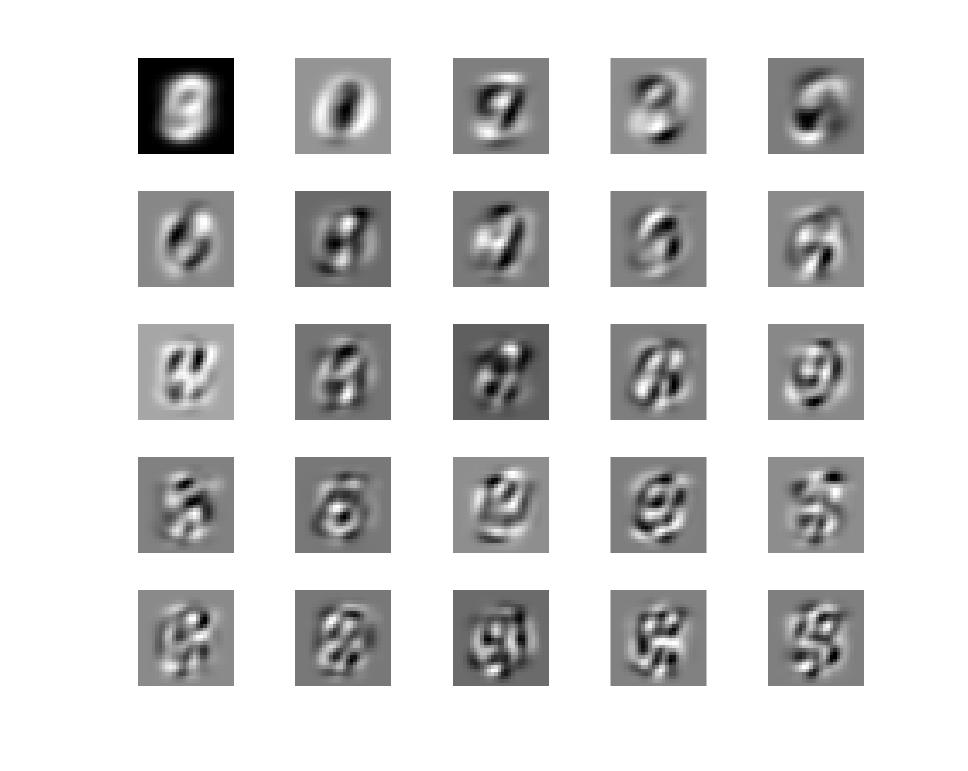
\includegraphics[width=5in]{U.jpg}}
    \caption{First 25 principal components of handwritten digit images (left to right, top to bottom)}
\end{figure}
First, let's check out our principle components here. The first principal components has a darker background than any other components, we can conclude that the first principle component is mainly about the background. \\
~\\
Based on the figure, we guess that the first ten principle components capture useful features of digits since we can vaguely see the shape of digits even though it is blurry. For example, the shape of digit 3 is captured by the fourth component. \\
~\\
Besides that, the rest of the principle components are chaotic, and we believe that they probably capture more detailed features and variations.
\newpage
\begin{figure}[h]
    \centerline{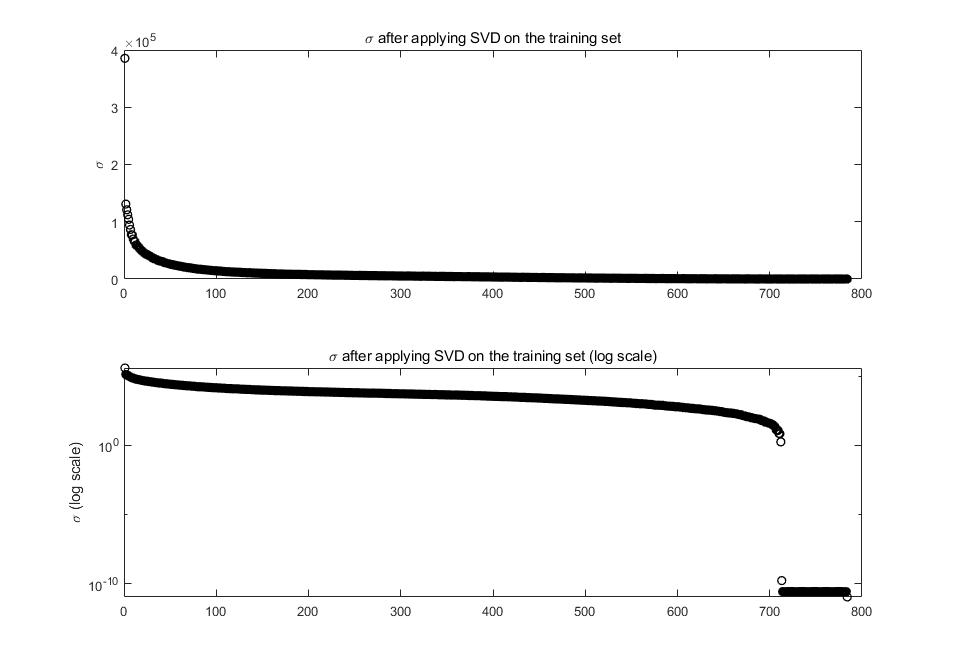
\includegraphics[width=5.5in]{S.jpg}}
    \caption{Singular values of handwritten digit images}
\end{figure}
From the figure, we can see that the first principles component carries lots of weight, which is expected since it captures the background shared in all images. The figure on the top tells us the first one hundred principle components carry quite significant amount of weights. When we zoomed in, the bottom figure shows that the singular value goes to 0 around 700. \\
~\\
\begin{figure}[h]
    \centerline{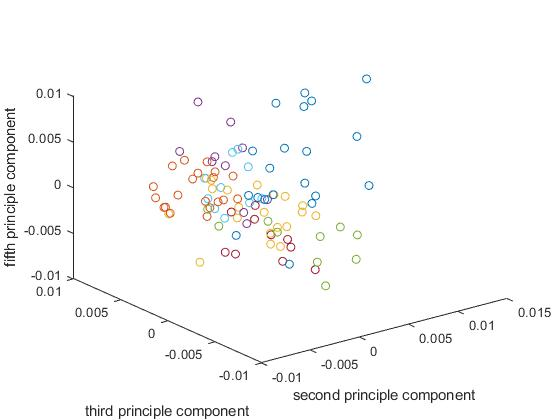
\includegraphics[width=2.5in]{V1.jpg}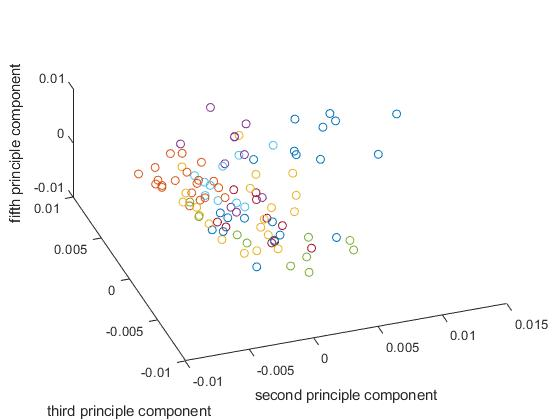
\includegraphics[width=2.5in]{V2.jpg}}
    \caption{Projection onto the second, third, and fifth components}
\end{figure}
~\\
Here, we project our data onto the second, third, and fifth components, and we only select 10 samples from each digit. The projections didn't give us a clear separation, except for blue dots. Obviously, 3 components is not enough for us to differentiate 10 groups.\\
~\\

\newpage
\subsection{Implementing the linear binary classifier}
Notice that, if we want to implement LDA, we need to find the principle components first. Since the goal is to implement a binary classifier, the principal components we got previously wouldn't be helpful, because it also captures the features of the digits we are not interested in. Therefore, we have to prepare a subset which contains only two digits. \\
~\\
The suitable threshold is determined by two pointer algorithm. Besides that, the rest of it is just calculations based on the formula and some small modifications. \\
~\\
Lastly, we wrote everything into a function so that we can test any specified pairs of digits. To illustrate its performance, we selected the digit pair 0 and 1.
\begin{algorithm}
\begin{algorithmic}
    \STATE{Prepare a subset that contains only two digits}
    \STATE{Apply the SVD and store principle component matrix $\mathbf{U}$}
    \STATE{Calculate $S_{between}$ and $S_{within}$}
    \STATE{Find the best projection vector $\mathbf{w}$}
    \IF{$\mu_1 < \mu_2$}
        \STATE{Set $\mathbf{w} = -\mathbf{w}$, making sure the first group tends to be smaller}
    \ENDIF
    \STATE{Find a suitable threshold}
\end{algorithmic}
\caption{Implementing the linear binary classifier}
\end{algorithm}
\begin{figure}[h]
    \centerline{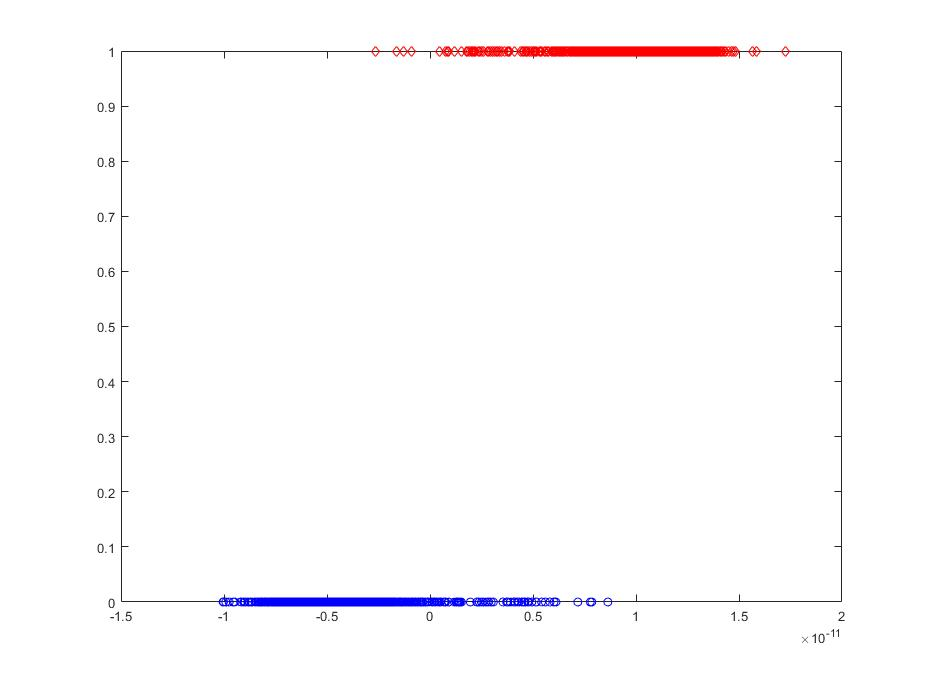
\includegraphics[width=3in]{LDA1.jpg}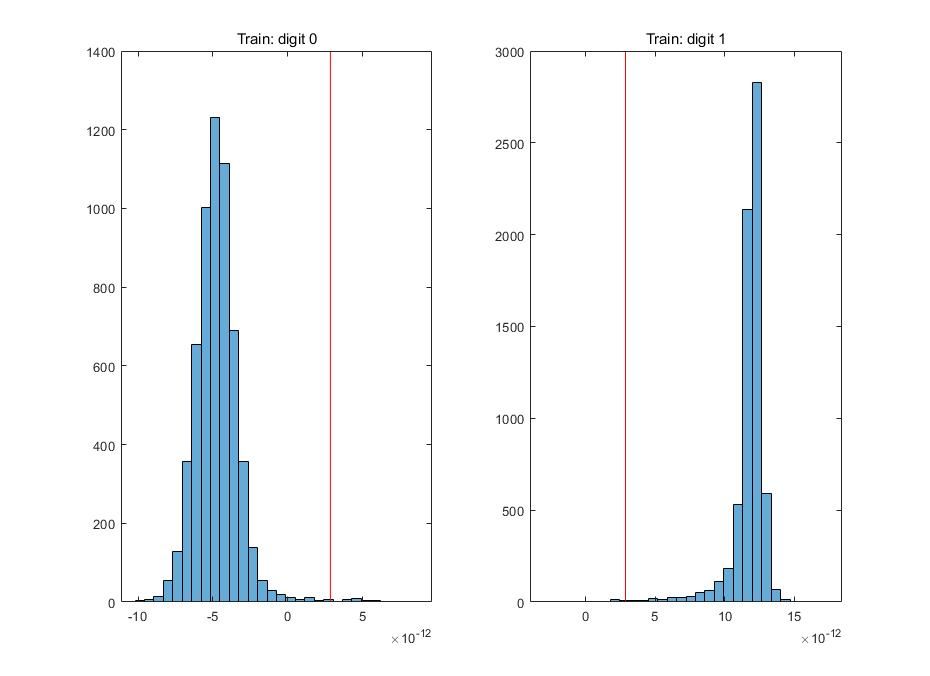
\includegraphics[width=3in]{LDA2.jpg}}
    \caption{The projection onto the vector $\mathbf{w}$ (left) The distribution of the projection and the threshold (right)}
\end{figure}
\subsection{Testing the linear binary classifier}
Similarly, to test the binary classifier we implemented, we also need to extract a subset from the testing set. Next, we calculate the projection by $\mathbf{V=U'X}$, and lastly, we determine the digit based on the threshold we found previously.
\begin{algorithm}
\begin{algorithmic}
    \STATE{Prepare a subset from the testing set that contains only two digits}
    \STATE{Calculate the projection by $\mathbf{V=U'X}$}
    \STATE{Identify the digits based on the threshold}
    \STATE{Calculate the accuracy}
\end{algorithmic}
\caption{Testing the linear binary classifier}
\end{algorithm}

\subsection{Implementing the linear trinary classifier}
The multi-class LDA is similar to the binary-class LDA, except for $S_{between}$ and $S_{within}$. Therefore, the major changes we made is updating the formula. \\
~\\
Moreover, the hardest part of this section is determining the thresholds. Since we have three digits now, therefore we need to find two suitable thresholds. The solution we give is applying the two pointer algorithm used in binary classifier twice. However, this algorithm requires the rank sequence of these three groups, which means that we have to check their projections and connect the interval with the digits manually. In this example, we select 0, 1, and 2 as our samples.\\
\begin{figure}[h]
    \centerline{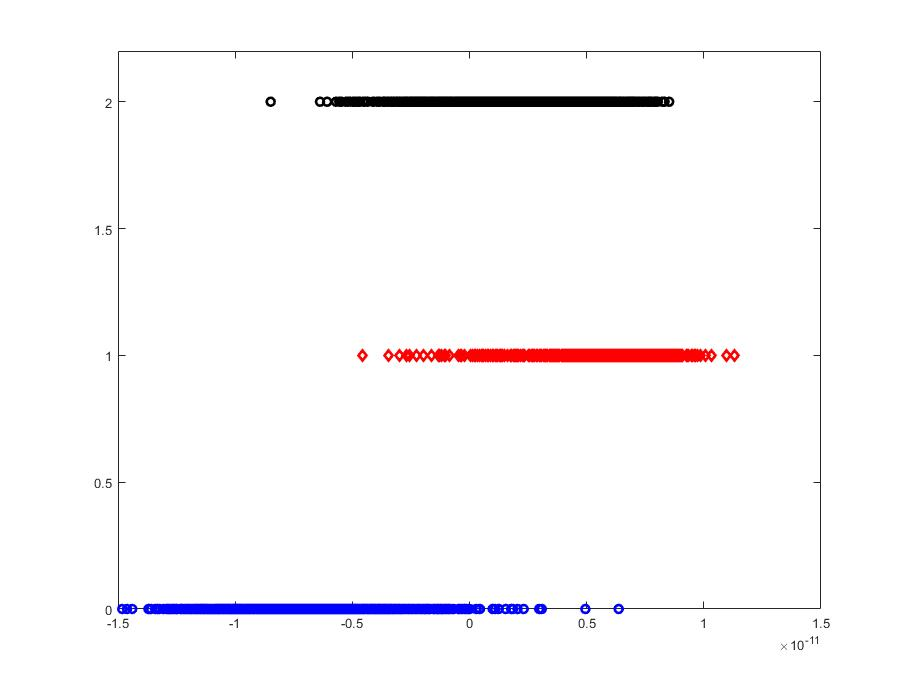
\includegraphics[width=3in]{LDA3.jpg}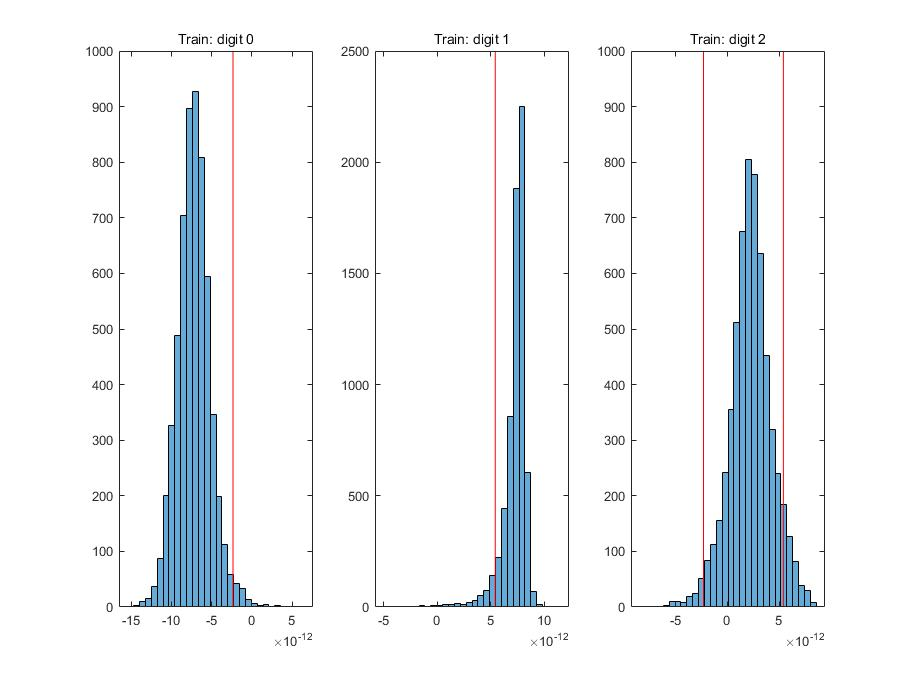
\includegraphics[width=3in]{LDA4.jpg}}
    \caption{The projection onto the vector $\mathbf{w}$ (left) The distribution of the projection and the threshold (right)}
\end{figure}


\subsection{Evaluating the performance of three binary classifiers}
In this section, we tested and compared three different binary classifiers: SVM, decision tree, and the linear classifier we implemented (LDA). Notice that, both the SVM and the decision tree are the built-in function in MATLAB, therefore we can implement them by simple call the functions. \\
~\\
To test their performance, we looped over all possible pairs of digits and generate an accuracy table.
\begin{algorithm}
\begin{algorithmic}
    \FOR{i=0:9}
        \FOR{j=i+1:9}
            \STATE{Train the classifiers by \texttt{fitctree} and \texttt{fitcsvm} on digits $i$ and $j$}
            \STATE{Find the prediction by \texttt{predict}}
            \STATE{Calculate the accuracy of identifying digit pair $i$ and $j$ for each classifier}
        \ENDFOR
    \ENDFOR
    \STATE{Find the minimum and the maximum accuracy by \texttt{min} and \texttt{max}}
\end{algorithmic}
\caption{Evaluating the performance of three binary classifiers}
\end{algorithm}

\section{Computational Result}
\subsection{Linear Discriminant Analysis}

Firstly, we tested the classifier we implemented. It scored higher than 0.96 on all pairs of digits. The digit pair of 3 and 5 is the most difficult to separate, and the accuracy is about 0.9634. the digit pair of 6 and 7 is the easiest to separate, and the accuracy is about 0.9993.\\
\begin{figure}[h]
    \centerline{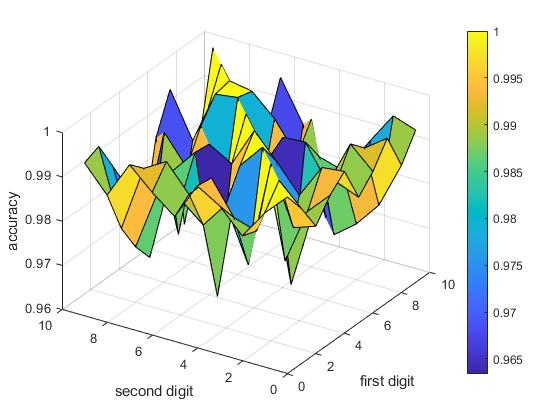
\includegraphics[width=3in]{surf1.jpg}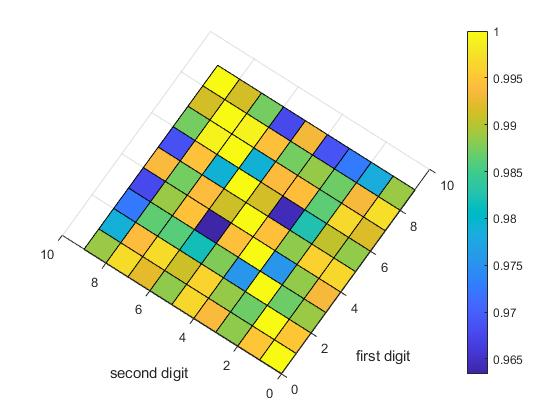
\includegraphics[width=3in]{surf2.jpg}}
    \caption{LDA: 3D visualization of the accuracy table}
\end{figure}
\begin{figure}[h]
    \centerline{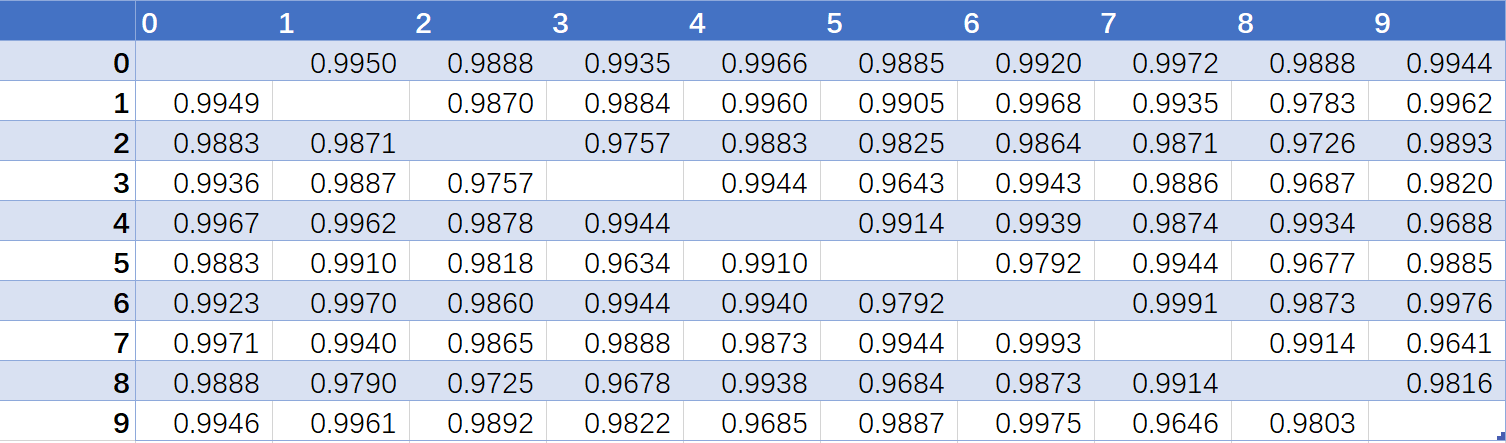
\includegraphics[width=6in]{LDAtable.PNG}}
    \caption{LDA: The accuracy table}
\end{figure}


\subsection{Decision Tree Classifiers}
As for the decision tree classifier, the overall accuracy is between 0.82 and 0.94. The pair with the highest accuracy is 0 and 1, and the pair with the lowest accuracy is 8 and 9.
\begin{figure}[h]
    \centerline{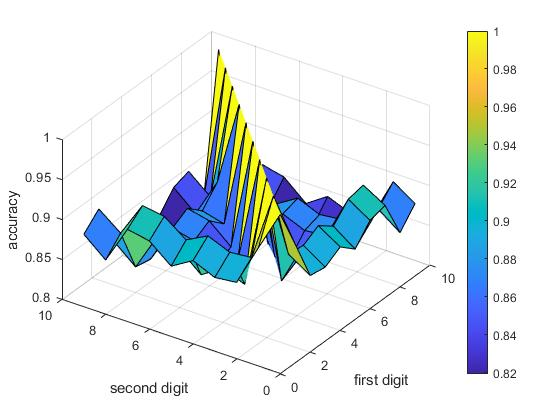
\includegraphics[width=3in]{surf3.jpg}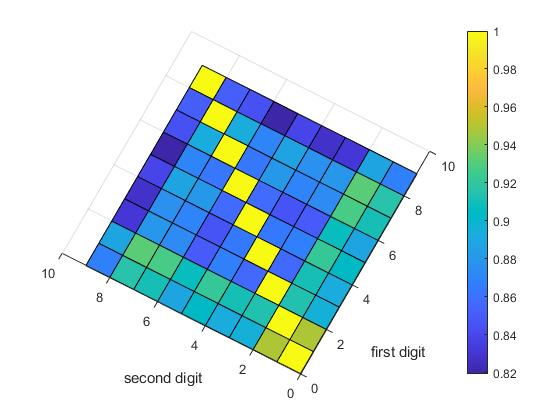
\includegraphics[width=3in]{surf4.jpg}}
    \caption{DTC: 3D visualization of the accuracy table}
\end{figure}
\begin{figure}[h]
    \centerline{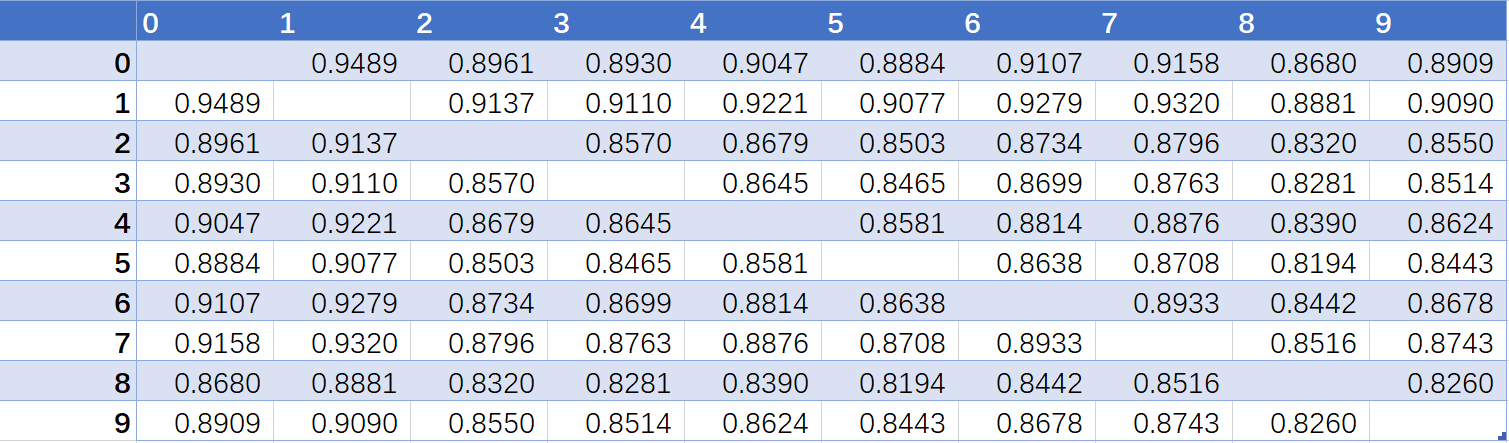
\includegraphics[width=6in]{DTCtable.PNG}}
    \caption{DTC: The accuracy table}
\end{figure}

\newpage
\subsection{Support Vector Machines}
As for the decision tree classifier, the overall accuracy is between 0.76 and 0.99. The best pair is  0 and 1, and the worst pair is 7 and 9.
\begin{figure}[h]
    \centerline{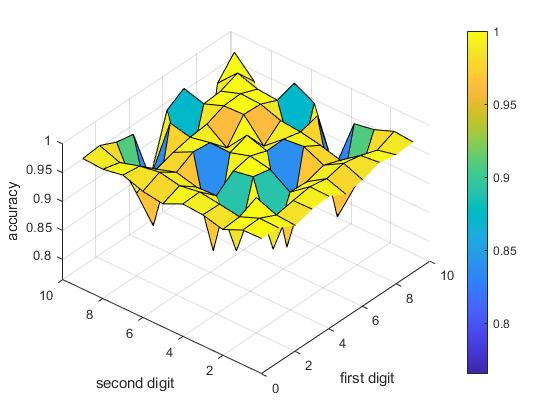
\includegraphics[width=3in]{surf5.jpg}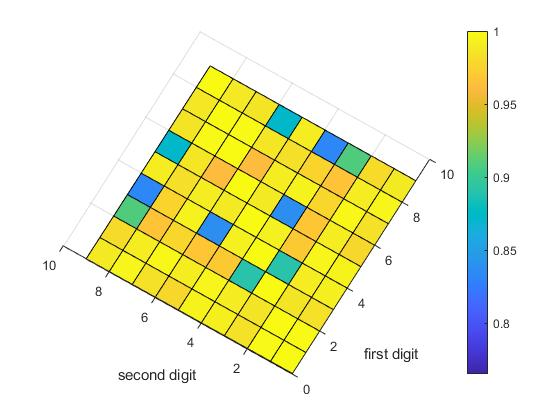
\includegraphics[width=3in]{surf6.jpg}}
    \caption{SVM: 3D visualization of the accuracy table}
\end{figure}
\begin{figure}[h]
    \centerline{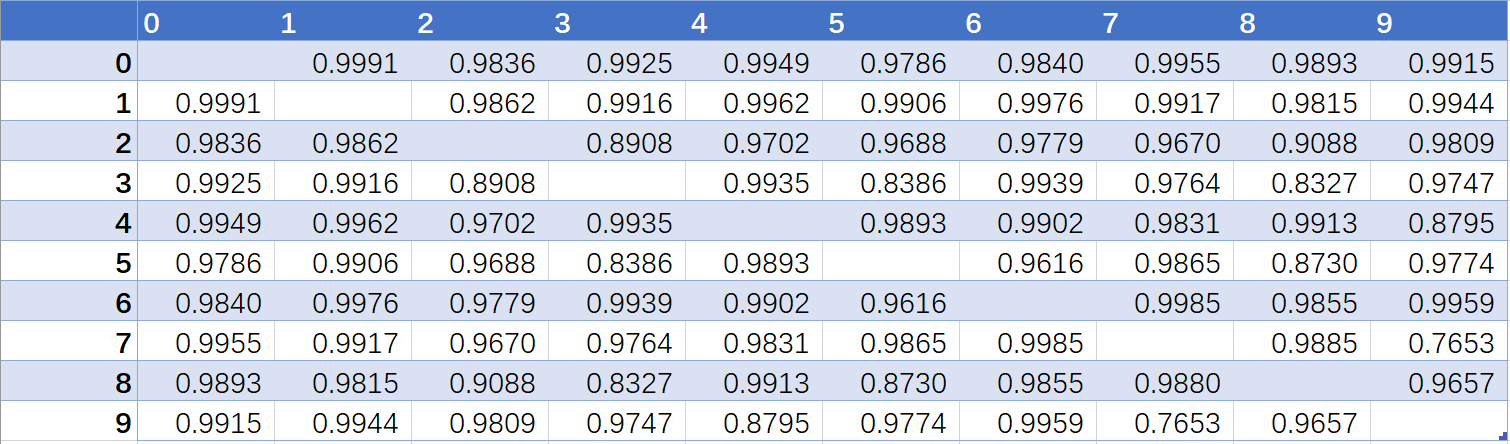
\includegraphics[width=6in]{SVMtable.PNG}}
    \caption{SVM: The accuracy table}
\end{figure}

\newpage

\section{Summary and Conclusion}
In the study, we applied the SVD to analyze the components, the weights, and the projections of these handwritten digit images. Moreover, we implemented LDA and LDS, creating a binary classier and a trinary classier. Lastly, we compared LDA with DTC and SVM. It turns out the classifier based on LDA is the best among three classier. SVM and DTC are the second and the third respectively. \\
~\\
% Appendices
\begin{appendices}

% MATLAB Functions
\section{MATLAB Functions}
\begin{itemize}
    \item \texttt{tree = fitctree(X,Y)} returns a fitted binary classification decision tree based on the input variables contained in matrix \mathbf{X} and output \mathbf{Y}. The returned binary tree splits branching nodes based on the values of a column of \mathbf{X}.
    \item \texttt{Mdl = fitcsvm(X,Y)} returns an SVM classifier trained using the predictors in the matrix \mathbf{X} and the class labels in vector \mathbf{Y} for one-class or two-class classification.
    \item \texttt{ypred = predict(mdl,Xnew)} returns the predicted response values of the linear regression model \mathbf{mdl} to the points in \mathbf{Xnew}.
\end{itemize}

% MATLAB Codes

\section{MATLAB Code}

\begin{verbatim}
clear all; close all; clc;

[data, train_labels] = mnist_parse('train-images.idx3-ubyte', 'train-labels.idx1-ubyte');

data = double(data);
data = data(:)';
train_images = reshape(data(:), [784, 60000]);
% train_images = train_images - repmat(mean(train_images, 1), 784, 1);


[data, test_labels] = mnist_parse('t10k-images.idx3-ubyte', 't10k-labels.idx1-ubyte');

data = double(data);
data = data(:)';
test_images = reshape(data(:), [784, 10000]);
% test_images = test_images - repmat(mean(test_images, 1), 784, 1);

    %% part 1.1-2
    [U, S, V] = svd(train_images, 'econ');

    %% check U
    for k = 1:25
        subplot(5,5,k)
        u = reshape(U(:,k), 28, 28);
        u = rescale(u);
        imshow(u)
    end

%% check S
close all;
s = diag(S);

figure(1)
subplot(2,1,1)
plot(s, 'ko','Linewidth',1)
ylabel('\sigma')
title('\sigma after applying SVD on the training set')

subplot(2,1,2)
semilogy(s,'ko','Linewidth',1)
ylabel('\sigma (log scale)')
title('\sigma after applying SVD on the training set (log scale)')
%% V
basis = [2,3,5];
digits = [];
for i = 1:10
   digit_label = find(train_labels == i-1);
   digits = [digits; digit_label(1:10)'];
end

v = V(:, basis);
for i = 1:10
    plot3(v(digits(i,:), 1), v(digits(i,:),2), v(digits(i,:),3), 'o'); hold on;
    xlabel('second principle component')
    ylabel('third principle component')
    zlabel('fifth principle component')
end

%% part 2.1
close all;
d1 = get_images_by_label(0, train_images, train_labels);
d2 = get_images_by_label(1, train_images, train_labels);

dt1 = get_images_by_label(0, test_images, test_labels);
dt2 = get_images_by_label(1, test_images, test_labels);

[U, w, threshold] = lda2d(d1, d2, 700);
accur = lda2d_test(dt1, dt2, U, w, threshold);

%% part 2.2
close all; clc;
d1 = get_images_by_label(0, train_images, train_labels);
d2 = get_images_by_label(1, train_images, train_labels);
d3 = get_images_by_label(2, train_images, train_labels);
[U, w, t1, t2] = lda3d(d1, d2, d3, 700);

%% part 2.3-4
% calculation
accur = ones(10);
for i = 1:10
    for j = 1:10
        if i == j
            continue
        end
        d1 = get_images_by_label(i-1, train_images, train_labels);
        d2 = get_images_by_label(j-1, train_images, train_labels);

        dt1 = get_images_by_label(i-1, test_images, test_labels);
        dt2 = get_images_by_label(j-1, test_images, test_labels);
        
        [U, w, threshold] = lda2d(d1, d2, 700);
        accur(i, j) = lda2d_test(d1, d2, U, w, threshold);
    end
end
%% plot
load('DTC_accur.mat');
load('SVM_accur.mat');

accur = SVM_accur;
[X,Y] = meshgrid(0:9,0:9);
surf(X, Y, accur);
colorbar
xlabel('first digit')
ylabel('second digit')
zlabel('accuracy')

%% find the min and amx
[Min, I] = min(accur(:));
[min_d1, min_d2] = ind2sub(size(accur),I);
accur_d = accur - diag(ones(1,10));
[Max, I] = max(accur_d(:));
[max_d1, max_d2] = ind2sub(size(accur_d),I);

%% part 2.5 DTC and SVM
DTC_accur = ones(10);
SVM_accur = ones(10);
for i = 0:9
    for j = 0:9
        if i == j
            continue
        end
        dtr1 = get_images_by_label(i, train_images, train_labels);
        dtr2 = get_images_by_label(j, train_images, train_labels);

        dte1 = get_images_by_label(i, test_images, test_labels);
        dte2 = get_images_by_label(j, test_images, test_labels);
        
        d_train = [dtr1, dtr2];
        l_train = [ones(1, size(dtr1, 2)) * (i), ones(1, size(dtr2, 2)) * (j)];

        d_test = [dte1, dte2];
        l_test = [ones(1, size(dte1, 2)) * (i), ones(1, size(dte2, 2)) * (j)];
        
        % DTC
        DTC = fitctree(d_train', l_train);
        p = predict(tree, d_test')';
        DTC_accur(i+1, j+1) = sum((p - l_test) == 0) / size(d_test, 2);

        % SVM
        %SVM = fitcsvm(d_train', l_train);
        %p = predict(SVM, d_test')';
        %SVM_accur(i, j) = sum((p - l_test) == 0) / size(d_test, 2);
    end
end



function mat = get_images_by_label(digit,images,labels)
    indices = labels == digit;
    mat = images(:, indices);
end

function [U, w,threshold] = lda2d(d1,d2,feature)
    n1 = size(d1,2);
    n2 = size(d2,2);

    [U,S,V] = svd([d1 d2],'econ');
    
    d = S*V';
    U = U(:,1:feature);
    
    d1 = d(1:feature, 1:n1);
    d2 = d(1:feature, n1+1:n1+n2);
    m1 = mean(d1,2);
    m2 = mean(d2,2);

    d1s = d1 - m1;
    d2s = d2 - m2;
    Sw = d1s*d1s' + d2s * d2s';
    Sb = (m1-m2)*(m1-m2)'; % between class

    [V2, D] = eig(Sb,Sw); % linear disciminant analysis
    [lambda, ind] = max(abs(diag(D)));
    w = V2(:,ind);
    w = w/norm(w,2);
    
    v1 = w'*d1;
    v2 = w'*d2;

    if mean(v1) > mean(v2)
        w = -w;
        v1 = -v1;
        v2 = -v2;
    end
    %figure(4)
    %plot(v1,0,'ob')
    %hold on
    %plot(v2,1,'dr')
    %ylim([0 1])

    % Find the threshold value

    s1 = sort(v1);
    s2 = sort(v2);

    t1 = length(s1);
    t2 = 1;
    while s1(t1) > s2(t2)
        t1 = t1 - 1;
        t2 = t2 + 1;
    end
    
    threshold = (s1(t1) + s2(t2))/2;

    % Plot histogram of results
    %figure(6)
    %subplot(1,2,1)
    %histogram(s1,30); hold on, plot([threshold threshold], [0 1400],'r')
    %title('Train: digit 0')
    %subplot(1,2,2)
    %histogram(s2,30); hold on, plot([threshold threshold], [0 3000],'r')
    %title('Train: digit 1')
end


function [U, w, t1, t2] = lda3d(d1,d2,d3, feature)
    n1 = size(d1,2);
    n2 = size(d2,2);
    n3 = size(d3,2);


    [U,S,V] = svd([d1 d2 d3],'econ');
    
    d = S*V';
    U = U(:,1:feature);
    
    d1 = d(1:feature, 1:n1);
    d2 = d(1:feature, n1+1:n1+n2);
    d3 = d(1:feature, n1+n2+1:n1+n2+n3);

    m1 = mean(d1,2);
    m2 = mean(d2,2);
    m3 = mean(d3,2);
    m = mean([d1,d2,d3],2);
    
    Sw = 0;
    for k = 1:n1
        Sw = Sw + (d1(:,k) - m1)*(d1(:,k) - m1)';
    end
    for k = 1:n2
        Sw =  Sw + (d2(:,k) - m2)*(d2(:,k) - m2)';
    end
    for k = 1:n3
        Sw =  Sw + (d3(:,k) - m3)*(d3(:,k) - m3)';
    end

    Sb = (m1-m)*(m1-m)' + (m2-m)*(m2-m)' + (m3-m)*(m3-m)';

    [V2, D] = eig(Sb,Sw); % linear disciminant analysis
    [lambda, ind] = max(abs(diag(D)));
    w = V2(:,ind);
    w = w/norm(w,2);
    
    v1 = w'*d1;
    v2 = w'*d2;
    v3 = w'*d3;


    plot(v1,0,'ob','Linewidth',2)
    hold on
    plot(v2,1,'dr','Linewidth',2)
    plot(v3,2,'ok','Linewidth',2)

    ylim([0 2.2])

    % Find the threshold value

    s1 = sort(v1);
    s2 = sort(v2);
    s3 = sort(v3);


    t1 = length(s3);
    t2 = 1;
    while s2(t1) > s3(t2)
        t1 = t1 - 1;
        t2 = t2 + 1;
    end
    
    th1 = (s2(t1) + s3(t2))/2;
    
    t1 = length(s1);
    t2 = 1;
    while s3(t1) > s1(t2)
        t1 = t1 - 1;
        t2 = t2 + 1;
    end
    
    th2 = (s3(t1) + s1(t2))/2;
    
    figure(5)
    subplot(1,3,1)
    histogram(s1,30); hold on, plot([th2 th2], [0 1000],'r')
    title('Train: digit 0')
    subplot(1,3,2)
    histogram(s2,30); hold on, plot([th1 th1], [0 2500],'r')
    title('Train: digit 1')
    subplot(1,3,3)
    histogram(s3,30); hold on, plot([th2 th2], [0 1000],'r'); plot([th1 th1], [0 1000],'r')
    title('Train: digit 2')
    
end


function accur = lda2d_test(d1, d2, U, w, threshold)
    feature = size(w, 1);
    
    n1 = size(d1,2);
    n2 = size(d2,2);
    
    d = U'*[d1 d2];
    U = U(:,1:feature);
    
    d1 = d(1:feature, 1:n1);
    d2 = d(1:feature, n1+1:n1+n2);
    
    s1 = sort(w'*d1);
    s2 = sort(w'*d2);
    
    count = sum(s1 < threshold) + sum(s2 > threshold);
    accur = count / (n1+n2);
    

    
end


function [imgs_train, labels] = mnist_parse(path_to_digits, path_to_labels)

% The function is curtesy of stackoverflow user rayryeng from Sept. 20,
% 2016. Link: https://stackoverflow.com/questions/39580926/how-do-i-load-in-the-mnist-digits-and-label-data-in-matlab

% Open files
fid1 = fopen(path_to_digits, 'r');

% The labels file
fid2 = fopen(path_to_labels, 'r');

% Read in magic numbers for both files
A = fread(fid1, 1, 'uint32');
magicNumber1 = swapbytes(uint32(A)); % Should be 2051
fprintf('Magic Number - imgs_train: %d\n', magicNumber1);

A = fread(fid2, 1, 'uint32');
magicNumber2 = swapbytes(uint32(A)); % Should be 2049
fprintf('Magic Number - Labels: %d\n', magicNumber2);

% Read in total number of imgs_train
% Ensure that this number matches with the labels file
A = fread(fid1, 1, 'uint32');
totalimgs_train = swapbytes(uint32(A));
A = fread(fid2, 1, 'uint32');
if totalimgs_train ~= swapbytes(uint32(A))
    error('Total number of imgs_train read from imgs_train and labels files are not the same');
end
fprintf('Total number of imgs_train: %d\n', totalimgs_train);

% Read in number of rows
A = fread(fid1, 1, 'uint32');
numRows = swapbytes(uint32(A));

% Read in number of columns
A = fread(fid1, 1, 'uint32');
numCols = swapbytes(uint32(A));

fprintf('Dimensions of each digit: %d x %d\n', numRows, numCols);

% For each image, store into an individual slice
imgs_train = zeros(numRows, numCols, totalimgs_train, 'uint8');
for k = 1 : totalimgs_train
    % Read in numRows*numCols pixels at a time
    A = fread(fid1, numRows*numCols, 'uint8');

    % Reshape so that it becomes a matrix
    % We are actually reading this in column major format
    % so we need to transpose this at the end
    imgs_train(:,:,k) = reshape(uint8(A), numCols, numRows).';
end

% Read in the labels
labels = fread(fid2, totalimgs_train, 'uint8');

% Close the files
fclose(fid1);
fclose(fid2);

end

\end{verbatim}


\end{appendices}

\end{document}
